\chapter{Approach}

\section{System context}

The reimbursement-tool interacts with multiple actors and other software interfaces. In this section those interactions will be defined in detail.

\subsection{Context diagram}

\begin{figure}[H]
    \centering
    \fbox{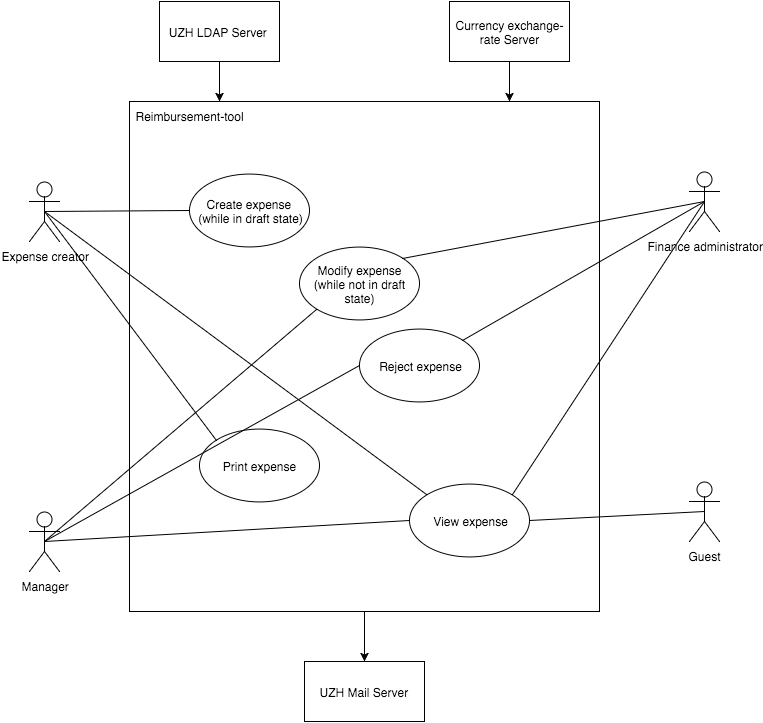
\includegraphics[width=0.80\textwidth]{context-diagram}}
    \caption{System context: Context diagram}
    \label{fig:context-diagram}
\end{figure}

The context diagram (see figure \ref{fig:context-diagram}) describes the important relationships between the system and its interrogators. \textit{Expense creator} such as normal employees or even professors can create expenses and print them. However, they are not allowed to modify an expense if it is not in draft state anymore. Further only managers and \textit{Finance admin} are allowed to \textit{Reject expenses} back to the \textit{Expense creator}.\newline
\textit{Guests} are allowed to view specific expenses. However, they need the 32-character long internal expense name id to gain access to it. This is only possible if a guest has access to the printed expense document. All other interrogators have access to all expenses they have to work with.

\subsubsection{LDAP dependency}

The system fetches the user data from the UZH-IFI LDAP server. This is necessary to synchronize the user database, to allow IFI users use the system without creating a new user name and password to access the systems functionality. Currently the synchronisation interval is defined to take part every 300 Seconds. By changing the 
value of \textit{reimbursement.ldap.refreshRate} on the file \textit{application.properties} stored at the 
back-end in the directory \textit{src/main/resources}. 

\section{Architecture}

The Back-end is considered as the software and database that runs on a server hosted by the IFI \cite{ifi}. The Front-end/client communicates with the Back-end using RESTful services described in section \ref{sec:restfulapi}.\newline

\subsection{Back-end}
The back-end is developed in Java. It is structured according to the rules of Domain Driven Design (DDD) \cite{ddd}. The domain model, that consists of the concepts, is connected to the database. Changes on the model will be automatically synchronized with the database. The service package lists all methods for a specific domain model.\newline DTOs (Data Transfer Object) are used to transfers data from back-end to front-end and vice verse. \newline The implemented model- and service-classes are visualized in the appendix \ref{sec:app-models} and \ref{sec:app-service}  

\subsection{Front-end}
The front-end is developed in JavaScript. It is based on the MVC (Model View Controller) pattern.   

\subsection{Multilayer architecture}
We use a common \textit{Multilayer architecture} (see figure \ref{fig:architecture-layer}) in the back-end to provide a good overview of the entire software-code. The following four layers are used:
\begin{itemize}
    \item \textbf{Presentation Layer} provides the front-end code for the GUI creation. It uses \textit{AngularJS} for the GUI creation. The \textit{Presentation Layer} interacts with the \textit{Application Layer}.
    \item \textbf{Application Layer} provides the available services that interact with the \textit{Business Layer}. It hosts the Security, RESTful services and the Global Exceptions.
    \item \textbf{Business Layer} provides the available services that interact with the \textit{Data Access Layer}. It provides the relevant services and models based on the \textit{Data Access Layer}.
    \item \textbf{Data Access Layer} consists of repositories and the \textit{Hybernate} database. 
\end{itemize}

\begin{figure}[H]
    \centering
    \fbox{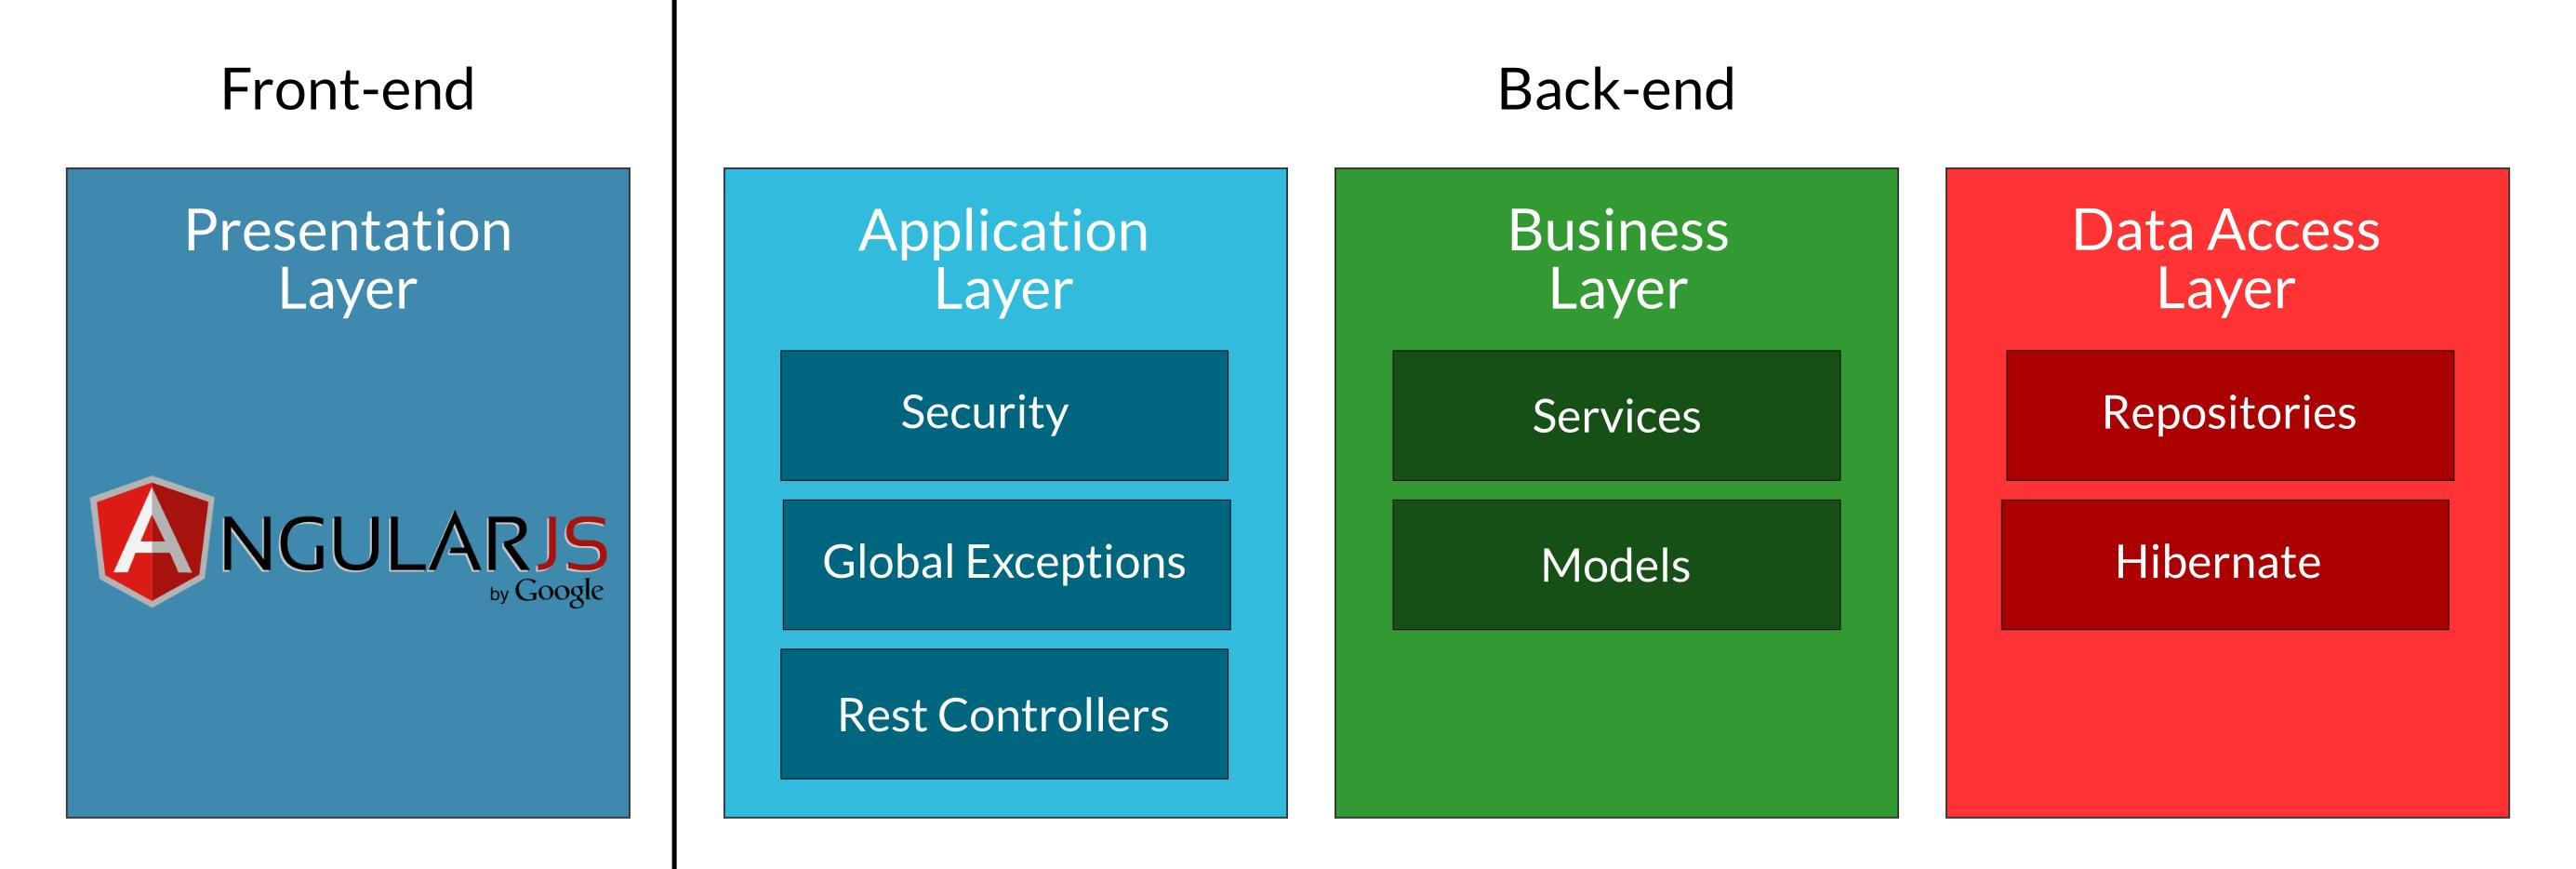
\includegraphics[width=0.80\textwidth]{architecture-layer}}
    \caption{Architecture: Multilayer architecture}
    \label{fig:architecture-layer}
\end{figure}

Our layers depend on each other while every layer communicates only with either the upper or the lower layer. This ensures a good maintainability and loose coupling of the single layers.\newline 
For example: If the presentation layer needs to display an expense, the application layer will handle this request by first checking the relevant security parameter of the request followed by calling the business layer. The service will handle and aggregate the desired information fetched from the relevant models. In our case to display an expense, the service will retrieve all expense-items and expense-item-attachments.


\subsection{Processflow}
\label{sec:processflow}
As described in \ref{sec:states} an expense is always in one specific state. The entire process implemented in the system is shown in figure \ref{fig:process-diagram}. The process is visualized using the BPML. Four lanes point out the available user roles. The process starts in the first lane; an expense is created, \textit{Receipts} are added and it is forwarded to the next higher instance for verification. After verifications by the \textit{Manager} or \textit{Department manager} and \textit{Finance administration} are successful, the user, \textit{Manager} and the \textit{Finance administration} needs to sign the document. If all users signed the document, it is ready to be printed by the user who created the expense.

\begin{figure}[H]
    \centering
    \fbox{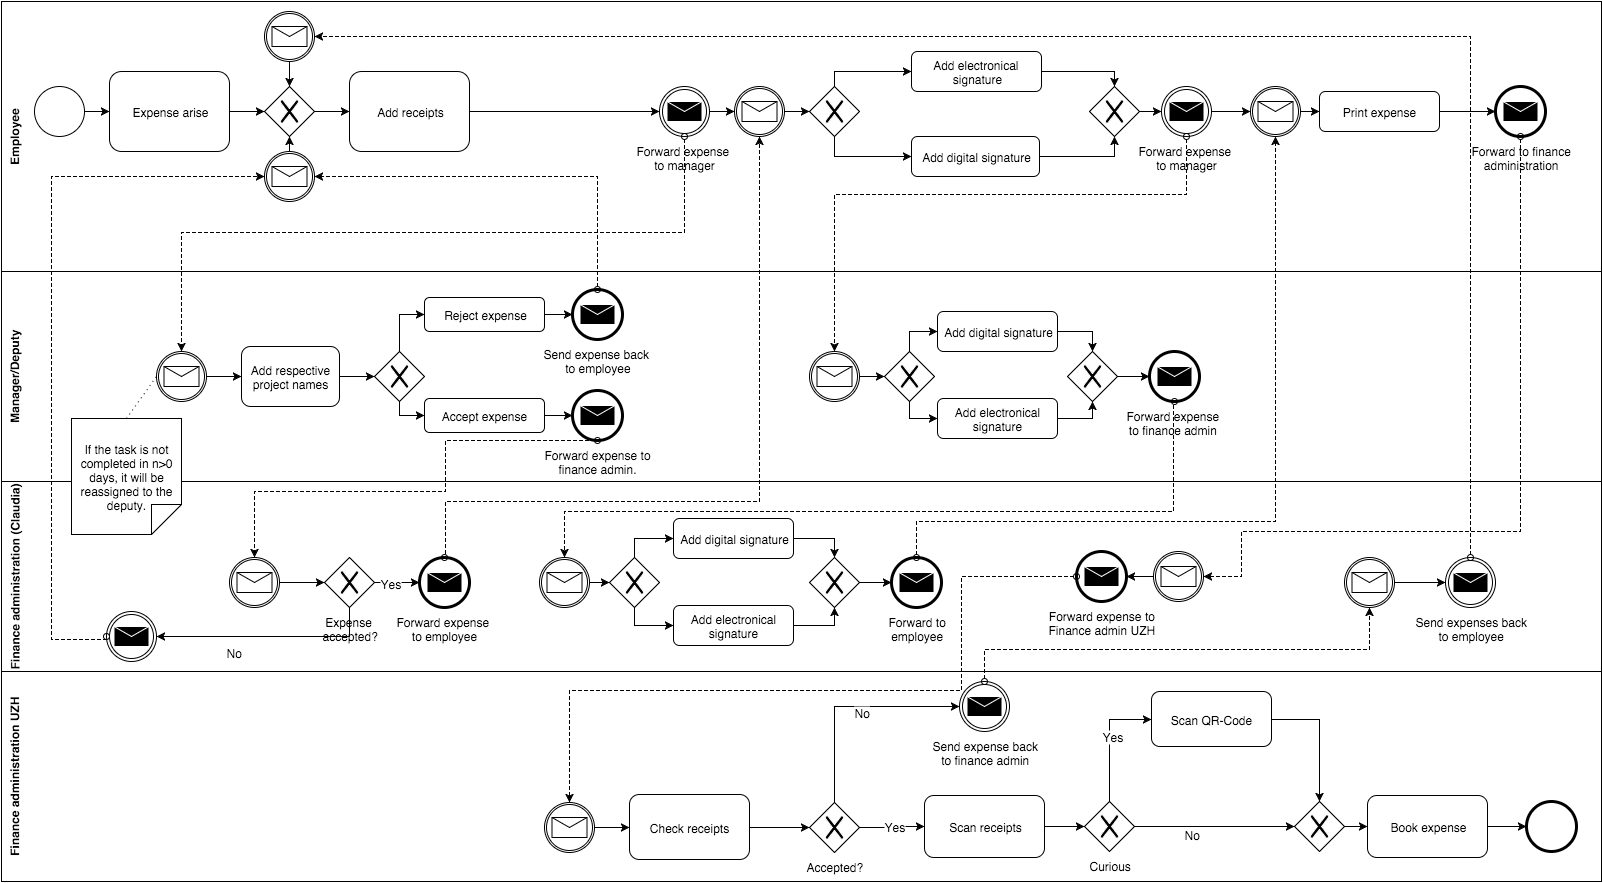
\includegraphics[width=0.80\textwidth]{process-diagram}}
    \caption{Architecture: Processflow}
    \label{fig:process-diagram}
\end{figure}


\section{Technologies}

In the following section the technologies used on the reimbursement-tool are being described detail.

\subsection{Back-end}

\subsubsection{Java}
The reimbursement-tool uses Java SE 7 for the Back-end programming language. Java is an industry wide standard, has detailed documentation and sufficient knowledge at the IFI \cite{ifi} department to guarantee an adequate support and future development of the software.

\subsubsection{Hibernate}
Hibernate abstracts the data layer. So that SQL-queries have to be written in rare cases only, which increases the code-clarity and decreases the code-complexity which can lead to bugs and errors. All data operation are handled implicitly by defined Java data classes.\newline
H2 database is a temporary database for storing data in a database environment. It offers a simple interface and can be used for developing, if only one development server database is available. \cite{hibernate}

\subsubsection{Java Spring Framework}
The reimbursement-tool uses various services of the Java Spring Framework \cite{spring}:
\begin{itemize}
    \item Spring Security for the login- and user-management as well as role based access-management for the RESTful resources.
    \item Spring Web MVC framework used to define RESTful interface within a few lines of code.
    \item Spring ORM used for the XML mapping within the process of Pdf-generation.
    \item Spring data is used to provide a simpler method to use data access technologies. It uses the DAO (Data Access Object) \cite{dao} to access data in a standard database like SQL. 
\end{itemize}

\subsubsection{Maven}
The tool uses Apache Maven \cite{maven} for the build process and dependency management.  

\subsubsection{Mockito}
The tool uses the Mockito framework to mock services. It can be used to write tests with a clean and simple API. Further it's easy to integrate with the Java Spring Testing framework. \cite{mockito}

\subsubsection{FOP-Apache}
After the process completion, the captured expenses need to printed on two A4 pages in landscape format. The structure of the sheets are predefined by the university. The generated Pdf by the reimbursement-tool needs to be identical to the existing MS-Office Excel file. See appendix \ref{sec:app-pdf} for the generated Pdf structure.\newline
The Pdf get generated using an individual created XSLT template and a XML document generated out of a Java Object. Combining these two files generates an FO document, which will be used by Apache FOP \cite{apache-fop} to generate a Pdf.\newline
We decided for Apache FOP because it is based on widely used standards like XML and XSL so that ongoing maintenance can be easily and without specific knowledge achieved.

\subsection{Interface}

\subsubsection{RESTful API}
\label{sec:restfulapi}
The tool uses a RESTful API that provides methods to access the Backend resources. It is implemented using the Spring MVC. 

\subsubsection{Swagger UI}
The Swagger UI visualizes all methods provided by the REST interface within a GUI. Furthermore developers can interact directly with the interface to test the methods. figure \ref{fig:swagger01} shows a screenshot of our used Swagger interface. It visualizes all the available methods for the \texttt{public} resource as well as the mandatory and optional parameters for \texttt{HTTP} calls. This was important for the process of development. \cite{swagger}

\begin{figure}[H]
    \centering
    \fbox{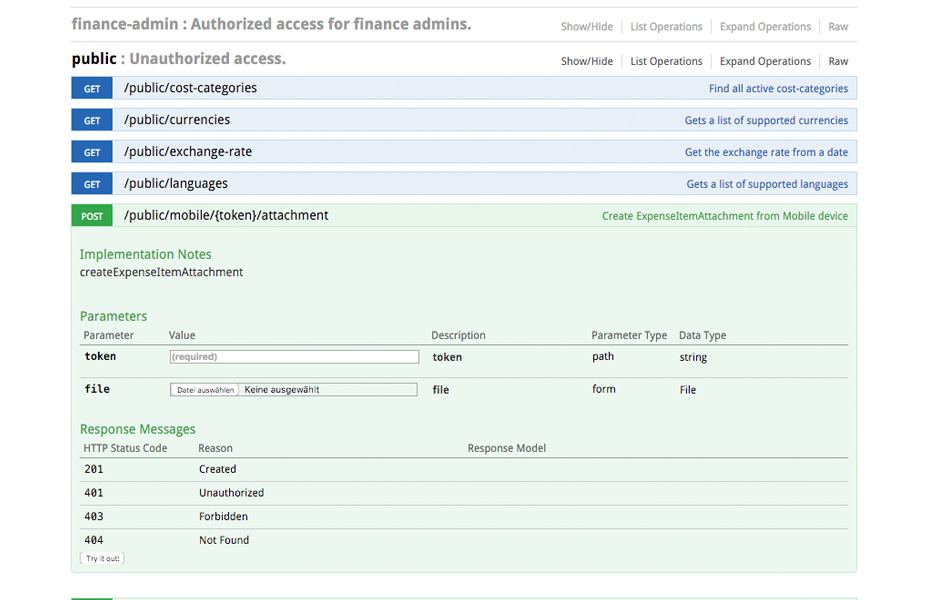
\includegraphics[width=0.80\textwidth]{swagger01}}
    \caption{Swagger: Reimbursement GUI}
    \label{fig:swagger01}
\end{figure}

\subsection{Front-end}

\subsubsection{AngularJS}
The tool uses the AngularJS framework for the client. Its data bindings and dependency injections reduces the amount of code need to be written. Further it uses HTML templates and a routing framework to create an interactive GUI. AngularJS is based on an MVC approach and is easy to integrate with REST services. \cite{angular}   

\subsubsection{Bootstrap}
Bootstrap is a framework that consists of HTML, CSS and JavaScript elements that can be used to create appealing responsive websites. It is supported by most of the desktop and mobile web browsers available. The tool uses Bootstrap v. 3.3.5. \cite{bootstrap}

\subsubsection{Bower}
The tool uses Bower for the client-side package management. Bower is a package manager for JavaScript web applications like AngularJS. It keeps track of the used assets, frameworks, libraries, etc. \cite{bower}  

\subsubsection{Grunt}
Grunt is a JavaScript task runner. We use it for our client-side build. Its plugin directory supports a lot of modules to optimize the development work flow. Code-uglifying, concating, sass-compiling, file operations, auto prefixing etc. \cite{grunt} 
